\section{Usability testing}
\label{usability}

The group first worked out a design prototype, and did a couple of internal usability tests. Afterwards we felt that our design was ready to be tested on external users. Ideally our external users would be doctors or other medical personnel, especially since these are the people who will be using our app, but because of a tight time schedule, and eagerness to complete all of the issues in sprint 2, our priority felt best used in completing the usability tests as quick as possible. This so that we could start  implementing the actual GUI. That’s why we did our usability tests on computer science students, among others.

Before we started the usability test we presented the intended area of use that our app would be operating, and asked the users to imagine themselves as a doctor or a radiologist. The compound scenario for the test was that you’d just completed examining a patient with the ultrasound device know as VScan. You are left with with three pictures you want to attach to the patients medical record. To attach these pictures with the current patient in the most easy way you decide to use our app.

We then presented our test subjects with four scenarios
\begin{itemize}
    \item Scenario 1 - User logs in: To log in to the application, the user must input a username (radiologist) and a password(abc).         Use this information to log in to our application.

    \item Scenario 2 - Choose pictures: You are prompted with a list of pictures from an earlier examination of a patient. You wish         to delete picture 1, and only use picture 3. 
    
    \item Scenario 3 - Look up patient. You know the social security number\\(12345678901) of your patient, and wish to use this number to look up the patient. 
    
	\item Scenario 4 - Upload results from an examination: You have chosen the pictures you wish to upload, and have identified your patient. You now wish to upload these pictures and in addition add a note that “It’s a boy”. Upload the pictures to the patients health record. 
\end{itemize}

\subsection{Views}

\begin{figure}[H]
\centering
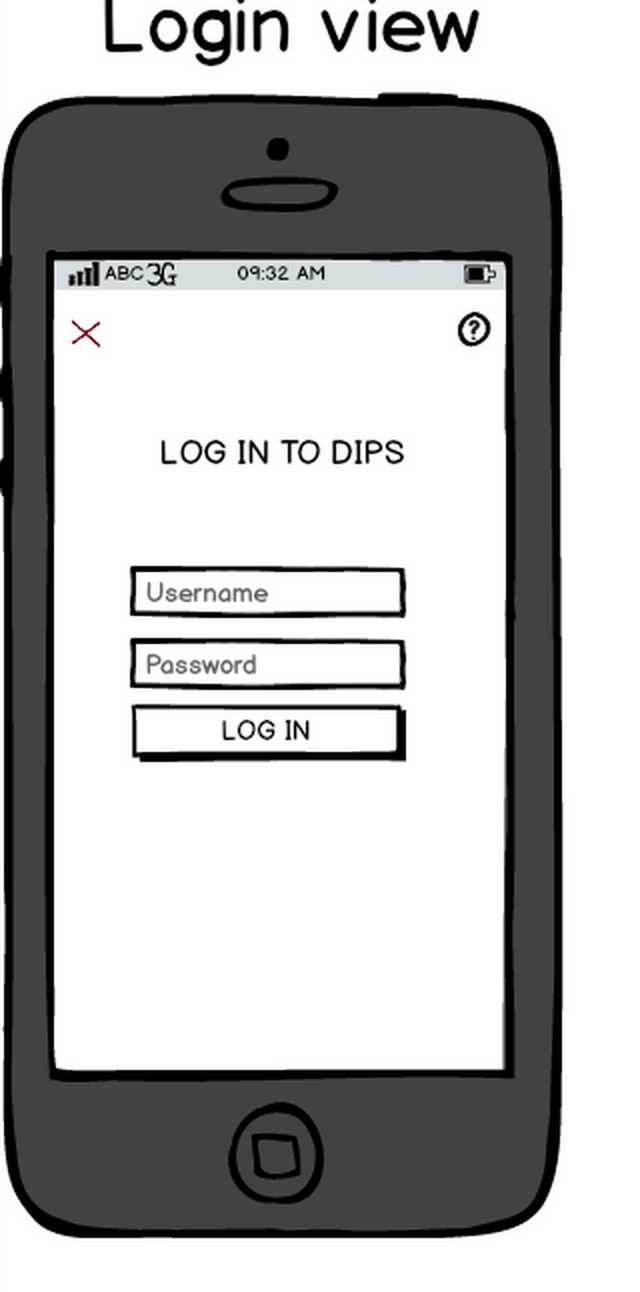
\includegraphics[scale=0.20]{img/mockups/login_view.png}
\caption{Login view}
\label{loginmock}
\end{figure}
We did not experience any issues while testing the login view (Figure \ref{loginmock}). As expected, the user clicked the username/password fields to input this information respectively. 


\begin{figure}[H]
\centering
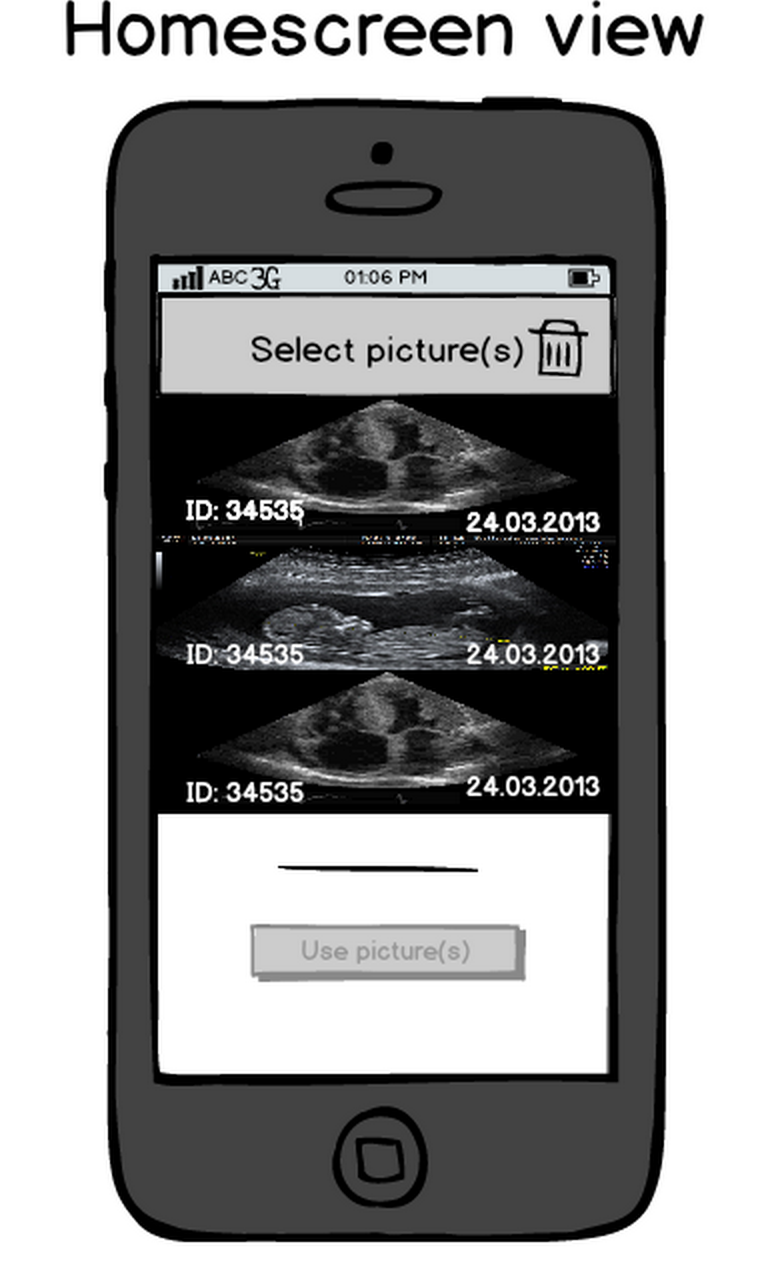
\includegraphics[scale=0.20]{img/mockups/homescreen_view.png}
\caption{Homescreen view}
\label{homemock}
\end{figure}
During testing of the home screen view (Figure \ref{homemock}), most users understood how to select the images. When they first understood how to select pictures, it seemed to be intuitive that they could delete them by selecting the delete icon, and in the same way choose which pictures to use, and proceed with the examination. 

\begin{figure}[H]
\centering
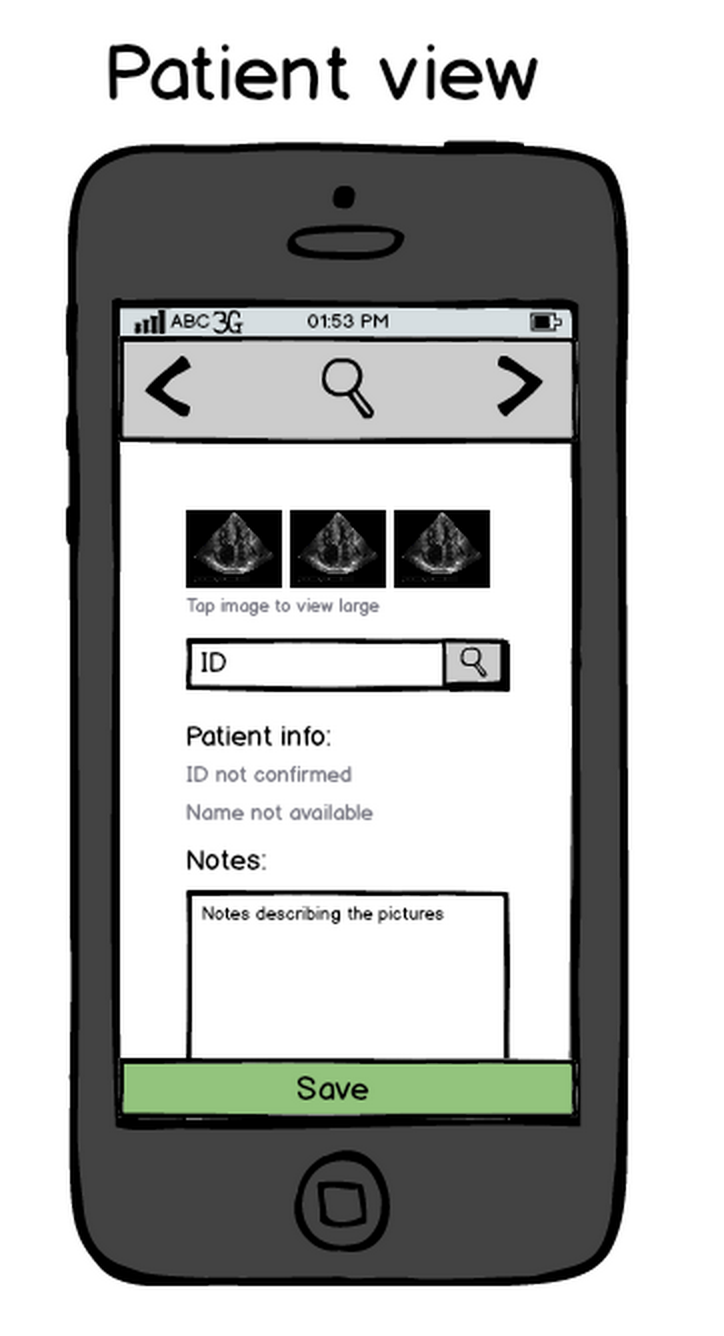
\includegraphics[scale=0.20]{img/mockups/patient_view.png}
\caption{Patient view}
\label{patientmock}
\end{figure}
We experienced several of our test subjects to be confused about the icons in the top left and right corner of the patient view (Figure \ref{patientmock}). In addition the magnifying glass icon made some subjects think that one could identify a patient by pressing it (as a button). 

\begin{figure}[H]
\centering
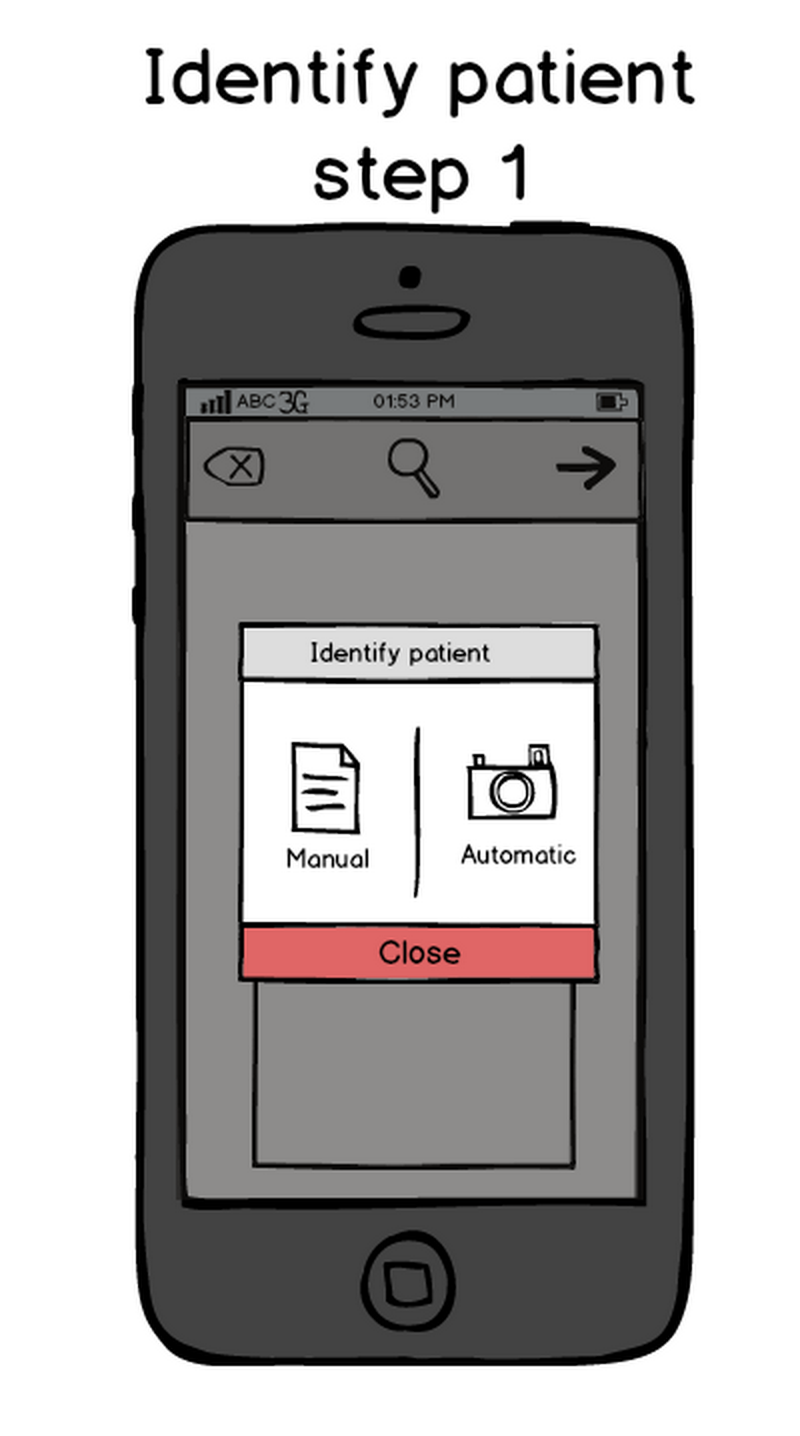
\includegraphics[scale=0.20]{img/mockups/identify_patient_1.png}
\caption{Identify patient view step 1}
\label{identifymock1}
\end{figure}
The identify patient view turned out be as intuitive as we wanted it to be. None of the test subjects appeared to have any problems using it. Nevertheless, we did (in retrospect) discover that the icons used could have been more self explaining. E.g. the automatic identification icon might have been more self explaining as a QR code icon, than a camera icon.

\begin{figure}[H]
\centering
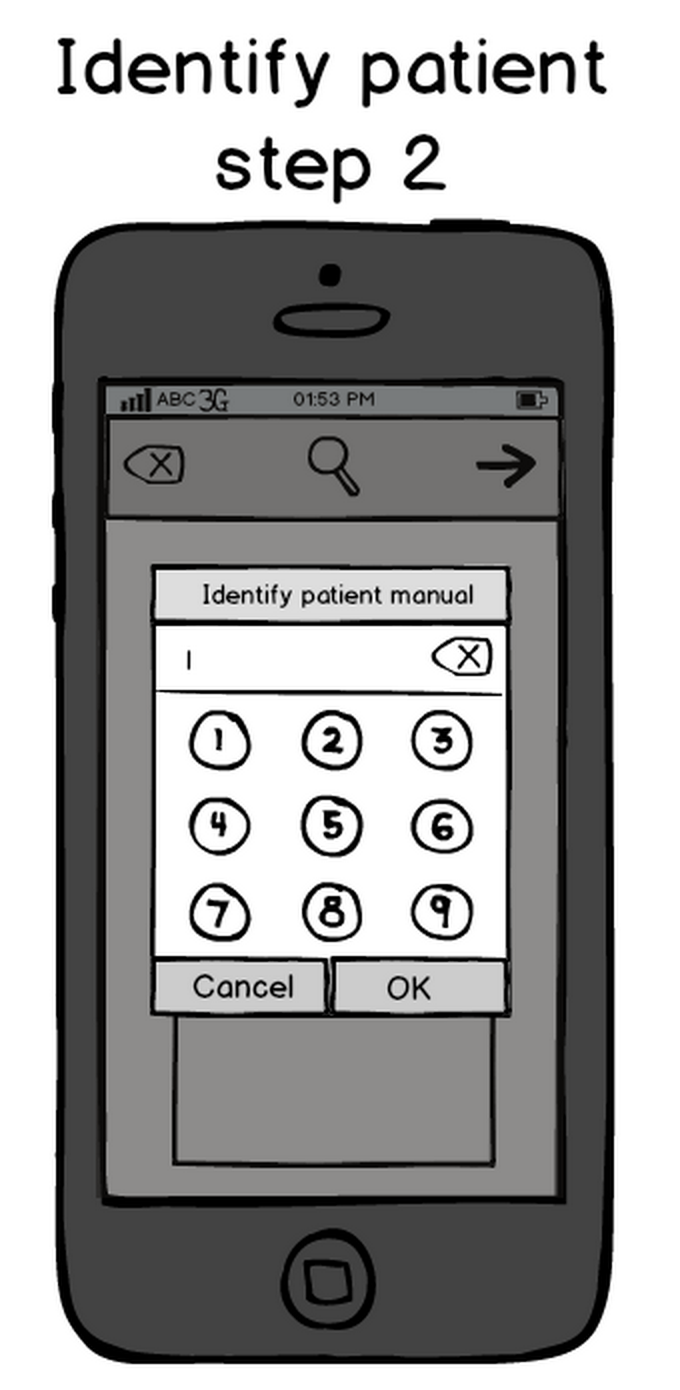
\includegraphics[scale=0.20]{img/mockups/identify_patient_2.png}
\caption{Identify patient view step 2}
\label{identifymock2}
\end{figure}
No issues were discovered while testing this view. The subjects understood that input was entered through the numerical keyboard on the screen.

\begin{figure}[H]
\centering
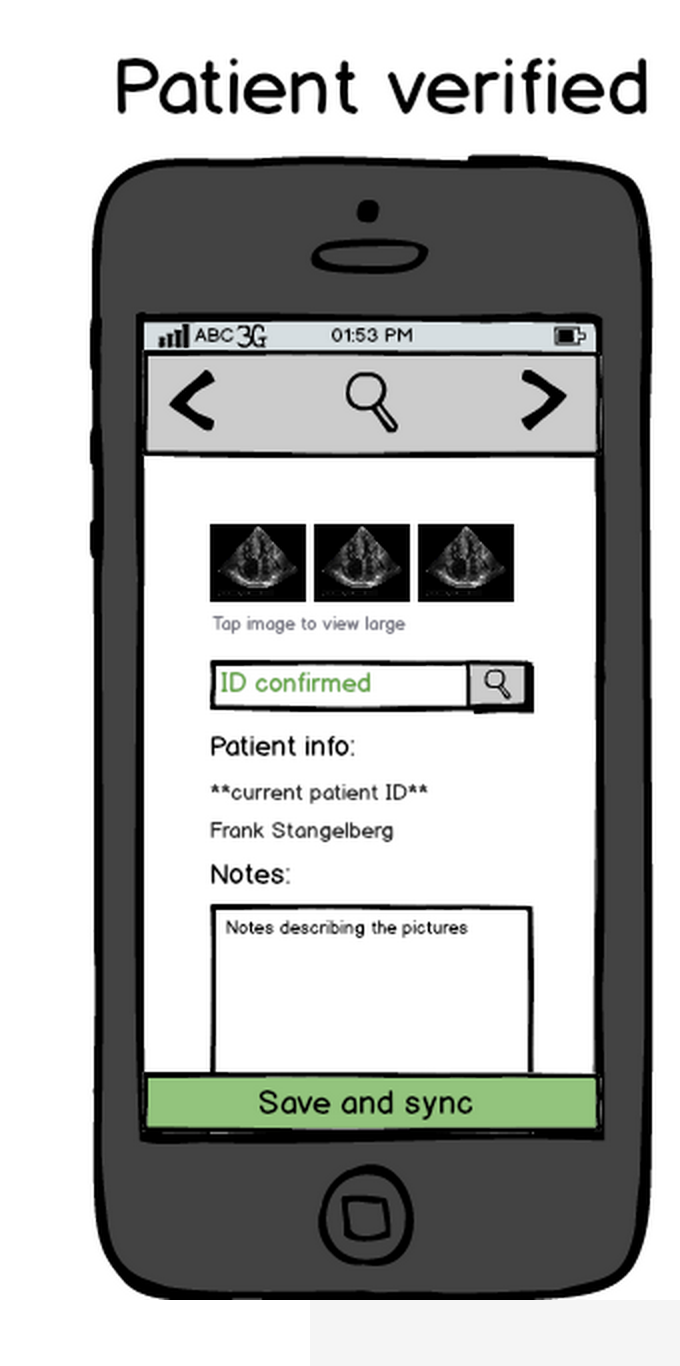
\includegraphics[scale=0.20]{img/mockups/patient_verified.png}
\caption{Patient verified view}
\label{verifymock}
\end{figure}
The patient verified view also had another problem after the patient had been identified. The “Save and sync” button at the bottom of the screen were not experienced as an actual button by the test subjects. To the contrary, this button was perceived as information.

\subsection{Conclusion}
During the usability test several potential issues were detected. Certain icons needs to be improved in order to meet the projects criteria for usability. We also established that the intended imaging functionality needs some adjustments in order to seem more intuitive and more easy to use. 

We feel that this round of usability tests have given us great feedback and insight in regards to how to proceed with our design. We were prepared to do a lot of changes in regards to how our design looked before the usability test, and as information and feedback was collected, did the respective changes which we felt was required. Our design now feels a lot more polished, but we’re prepared to do changes to make it as close to perfect as it can be.
